% ------------------------------------------------------------------------------
% TYPO3 CMS 7.0 - What's New - Chapter "Deprecated Functions" (English Version)
%
% @author	Michael Schams <schams.net>
% @license	Creative Commons BY-NC-SA 3.0
% @link		http://typo3.org/download/release-notes/whats-new/
% @language	English
% ------------------------------------------------------------------------------
% LTXE-CHAPTER-UID:		89070805-31adaab7-4f29d2f6-90399484
% LTXE-CHAPTER-NAME:	Deprecated Functions
% ------------------------------------------------------------------------------
% LTXE-SLIDE-START
% LTXE-SLIDE-UID:		c47248f9-03aa1da2-8dd9985d-762cf405
% LTXE-SLIDE-ORIGIN:	xxxxxxxx-xxxxxxxx-xxxxxxxx-xxxxxxxx
% LTXE-SLIDE-TITLE:		Legacy Layer
% LTXE-SLIDE-REFERENCE:	http://typo3.org/news/article/retaining-compatibility-to-typo3-cms6/
% ------------------------------------------------------------------------------

\begin{frame}[fragile]
	\frametitle{Deprecated/Removed Functions}
	\framesubtitle{Compatibility Layer}

	\begin{itemize}

		\item TYPO3 CMS 6.2: a compatiblity layer makes sure, old extensions work in the new codebase\newline
			\small
				Drawback: decreased performance (not the full potential of the system)
			\normalsize

		\item TYPO3 CMS 7.0: compatibility layer has been removed from the core\newline
			\small
				Impact: old extensions possibly break (e.g. extensions without namespaces)
			\normalsize

		\item Compatibility can be re-inforced by installing system extension \texttt{EXT:compatibility6} if required
		\item This extension will be moved to TER at one point in the future

	\end{itemize}

\end{frame}

% ------------------------------------------------------------------------------
% LTXE-SLIDE-START
% LTXE-SLIDE-UID:		70da8aab-cd42e15f-fe254b81-41ceabb5
% LTXE-SLIDE-ORIGIN:	xxxxxxxx-xxxxxxxx-xxxxxxxx-xxxxxxxx
% LTXE-SLIDE-TITLE:		Backend User Management
% ------------------------------------------------------------------------------

\begin{frame}[fragile]
	\frametitle{Deprecated/Removed Functions}
	\framesubtitle{Backend User Management}

	\begin{itemize}
		\item Switch to backend user ("change-to mode") has been removed
	\end{itemize}

	\smaller\tabto{1cm}\begingroup\color{typo3red}TYPO3 CMS 6.2\endgroup\normalsize
	\begin{figure}\vspace{-0.4cm}
		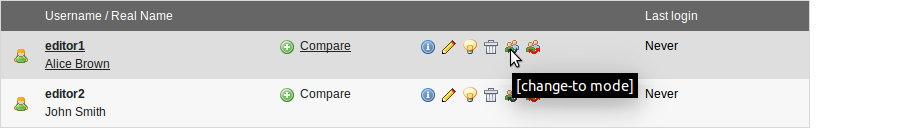
\includegraphics[width=0.90\linewidth]{DeprecatedRemovedFunctions/BackendUserSwitch1.png}
	\end{figure}

	\smaller\tabto{1cm}\begingroup\color{typo3red}TYPO3 CMS 7.0\endgroup\normalsize
	\begin{figure}\vspace{-0.4cm}
		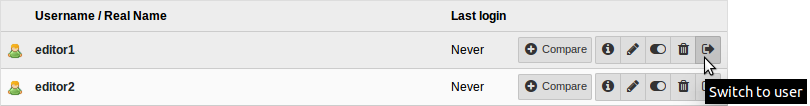
\includegraphics[width=0.90\linewidth]{DeprecatedRemovedFunctions/BackendUserSwitch2.png}
	\end{figure}

\end{frame}

% ------------------------------------------------------------------------------
% LTXE-SLIDE-START
% LTXE-SLIDE-UID:		10805d4d-787ce2f8-10e4329a-1451521a
% LTXE-SLIDE-ORIGIN:	xxxxxxxx-xxxxxxxx-xxxxxxxx-xxxxxxxx
% LTXE-SLIDE-TITLE:		Removed Deprecated JavaScript Functions
% LTXE-SLIDE-REFERENCE:	https://github.com/TYPO3/TYPO3.CMS/commit/2dff81b963e1b77c7f068f91ffde73914a18b0be
% LTXE-SLIDE-REFERENCE:	https://forge.typo3.org/issues/62291
% LTXE-SLIDE-REFERENCE:	https://forge.typo3.org/projects/typo3cms-core/repository/revisions/9ac03e383e4786e868f4b1d81893e84c4621abc8/entry/typo3/sysext/core/Documentation/Changelog/master/Breaking-62291-RTEDeprecatedJavaScriptMethodsRemoved.rst
% ------------------------------------------------------------------------------

\begin{frame}[fragile]
	\frametitle{Deprecated/Removed Functions}
	\framesubtitle{Removed Deprecated JavaScript Functions}

	\begin{itemize}
		\item In accordance with the \href{http://forge.typo3.org/projects/typo3v4-core/wiki/CoreDevPolicy}{deprecation strategy},
			a number of JavaScript methods, classified as \textit{deprecated} since TYPO3 CMS 4.7, have been removed, for example:

		\begin{lstlisting}
			\TYPO3\CMS\Backend\Form\FormEngine->getSingleField_typeInput
			\TYPO3\CMS\Backend\Form\FormEngine->getSingleField_typeText
			\TYPO3\CMS\Core\Utility\GeneralUtility->quoted_printable
			\TYPO3\CMS\Core\Utility\GeneralUtility->encodeHeader
		\end{lstlisting}

		\smaller
			\texttt{HTMLArea.Editor.forceRedraw}\newline
				(use \texttt{HTMLArea.Framework.doLayout} instead)
				\vspace{0.2cm}

			\texttt{HTMLArea.Editor.convertNode}\newline
				(use \texttt{HTMLArea.DOM.convertNode} instead)
				\vspace{0.2cm}

			\texttt{HTMLArea.Editor.getBlockAncestors}\newline
				(use \texttt{HTMLArea.DOM.getBlockAncestors} instead)
		\normalsize

	\end{itemize}

\end{frame}

% ------------------------------------------------------------------------------
% LTXE-SLIDE-START
% LTXE-SLIDE-UID:		9da41efc-970e66a8-f9163c40-67cfa712
% LTXE-SLIDE-ORIGIN:	xxxxxxxx-xxxxxxxx-xxxxxxxx-xxxxxxxx
% LTXE-SLIDE-TITLE:		Removed Functions (1)
% LTXE-SLIDE-REFERENCE:	https://forge.typo3.org/issues/17579
% LTXE-SLIDE-REFERENCE:	https://forge.typo3.org/issues/62888
% ------------------------------------------------------------------------------

\begin{frame}[fragile]
	\frametitle{Deprecated/Removed Functions}
	\framesubtitle{Removed Functions (1)}

	\begin{itemize}

		\item
			\small
				TypoScript setting \texttt{config.uniqueLinkVars} has been removed\newline
				(this behaviour is the default now)
			\normalsize

		\item
			\small
				ViewHelper
					\texttt{\textbackslash
						TYPO3\textbackslash
						CMS\textbackslash
						Documentation\textbackslash
						ViewHelpers\textbackslash
						Link\textbackslash
						Action}
					has been removed (use \texttt{f:be.buttons.icon} or \texttt{f:uri.*} instead)
			\normalsize

		\item
			\small
				PageTSconfig option \texttt{mod.web\_list.alternateBgColors}\newline
				has been removed
			\normalsize

		\item
			\small
				PropertyMapper has been removed\newline
				(including option \texttt{rewrittenPropertyMapper = 0})
			\normalsize

		\item
			\small
				TypoScript conditions have been removed:

					\begin{itemize}
						\item\texttt{browser}
						\item\texttt{version}
						\item\texttt{system}
						\item\texttt{useragent}
					\end{itemize}
			\normalsize

	\end{itemize}

\end{frame}

% ------------------------------------------------------------------------------
% LTXE-SLIDE-START
% LTXE-SLIDE-UID:		efe86631-b6020ae8-ffa01160-6de29dc3
% LTXE-SLIDE-ORIGIN:	xxxxxxxx-xxxxxxxx-xxxxxxxx-xxxxxxxx
% LTXE-SLIDE-TITLE:		Removed Methods (1)
% ------------------------------------------------------------------------------

\begin{frame}[fragile]
	\frametitle{Deprecated/Removed Functions}
	\framesubtitle{Removed Methods (1)}

	The following \textbf{methods} have been removed:

	\begin{itemize}
		\item
			\small
				\texttt{connectDB}\newline
				of class
				\texttt{\textbackslash
					TYPO3\textbackslash
					CMS\textbackslash
					Frontend\textbackslash
					Utility\textbackslash
					EidUtility}
			\normalsize
		\item
			\small
				\texttt{isDisplayCondition}\newline
				of class
				\texttt{\textbackslash
					TYPO3\textbackslash
					CMS\textbackslash
					Form\textbackslash
					FormEngine}
			\normalsize
		\item
			\small
				\texttt{int\_from\_ver}\newline
				of class
				\texttt{\textbackslash
					TYPO3\textbackslash
					CMS\textbackslash
					Core\textbackslash
					Utility\textbackslash
					GeneralUtility}
			\normalsize
		\item
			\small
				\texttt{getUniqueFields}\newline
				of class
				\texttt{\textbackslash
					TYPO3\textbackslash
					CMS\textbackslash
					Core\textbackslash
					DataHandling\textbackslash
					DataHandler}
			\normalsize

	\end{itemize}

\end{frame}

% ------------------------------------------------------------------------------
% LTXE-SLIDE-START
% LTXE-SLIDE-UID:		293414d4-e87db3d5-afced471-ca9826ed
% LTXE-SLIDE-ORIGIN:	xxxxxxxx-xxxxxxxx-xxxxxxxx-xxxxxxxx
% LTXE-SLIDE-TITLE:		Removed Methods (2)
% ------------------------------------------------------------------------------

\begin{frame}[fragile]
	\frametitle{Deprecated/Removed Functions}
	\framesubtitle{Removed Methods (2)}

	The following \textbf{methods} have been removed:

	\begin{itemize}

		\item
			\small
				\texttt{isSafeModeEnabled}\newline
				of class
				\texttt{\textbackslash
					TYPO3\textbackslash
					CMS\textbackslash
					Core\textbackslash
					Utility\textbackslash
					PhpOptionsUtility}
			\normalsize
		\item
			\small
				\texttt{registerSwiftMailer}\newline
				of class
				\texttt{\textbackslash
					TYPO3\textbackslash
					CMS\textbackslash
					Core\textbackslash
					Bootstrap}
			\normalsize
		\item
			\small
				\texttt{loadTCA}\newline
				of class
				\texttt{\textbackslash
					TYPO3\textbackslash
					CMS\textbackslash
					Core\textbackslash
					Utility\textbackslash
					GeneralUtility}
			\normalsize
		\item
			\small
				\texttt{isLocalconfWritable}\newline
				of class
				\texttt{\textbackslash
					TYPO3\textbackslash
					CMS\textbackslash
					Core\textbackslash
					Utility\textbackslash
					ExtensionManagementUtility}
			\normalsize

	\end{itemize}

\end{frame}

% ------------------------------------------------------------------------------
% LTXE-SLIDE-START
% LTXE-SLIDE-UID:		a1ba1998-f88c1063-71470741-30b9f314
% LTXE-SLIDE-ORIGIN:	xxxxxxxx-xxxxxxxx-xxxxxxxx-xxxxxxxx
% LTXE-SLIDE-TITLE:		Removed Classes
% ------------------------------------------------------------------------------

\begin{frame}[fragile]
	\frametitle{Deprecated/Removed Functions}
	\framesubtitle{Removed Classes}

	The following \textbf{classes} have been removed:

	\begin{itemize}

		\item
			\smaller
				\texttt{\textbackslash
					TYPO3\textbackslash
					CMS\textbackslash
					Backend\textbackslash
					Template\textbackslash
					MediumDocumentTemplate}
			\normalsize
		\item
			\smaller
				\texttt{\textbackslash
					TYPO3\textbackslash
					CMS\textbackslash
					Extbase\textbackslash
					Service\textbackslash
					TypeHandlingService}
			\normalsize

	\end{itemize}

\end{frame}

% ------------------------------------------------------------------------------
